\documentclass[12pt, titlepage]{article}

\usepackage{fullpage}
\usepackage[round]{natbib}
\usepackage{multirow}
\usepackage{booktabs}
\usepackage{tabularx}
\usepackage{graphicx}
\usepackage{float}
\usepackage{hyperref}
\hypersetup{
    colorlinks,
    citecolor=blue,
    filecolor=black,
    linkcolor=red,
    urlcolor=blue
}

\newcounter{acnum}
\newcommand{\actheacnum}{AC\theacnum}
\newcommand{\acref}[1]{AC\ref{#1}}

\newcounter{ucnum}
\newcommand{\uctheucnum}{UC\theucnum}
\newcommand{\uref}[1]{UC\ref{#1}}

\newcounter{mnum}
\newcommand{\mthemnum}{M\themnum}
\newcommand{\mref}[1]{M\ref{#1}}

\begin{document}



\title{\textbf{yoGERT GIS Toolbox}\\ Capstone 4G06\\ System Design Document}
\author{Team 19,
		\\ Smita Singh, Abeer Alyasiri, Niyatha Rangarajan,\\ Moksha Srinivasan, Nicholas Lobo, Longwei Ye \\\\
}
\date{\today}

\maketitle

\pagenumbering{roman}

\section{Revision History}

\begin{tabularx}{\textwidth}{p{3cm}p{2cm}X}
\toprule {\bf Date} & {\bf Version} & {\bf Notes}\\
\midrule
January 10th, 2023 & 1.0 & Updated Sections 2-11\\
\bottomrule
\end{tabularx}

\newpage

\section{Reference Material}

This section records information for easy reference.

\subsection{Abbreviations and Acronyms}

\renewcommand{\arraystretch}{1.2}
\begin{tabular}{l l} 
  \toprule		
  \textbf{symbol} & \textbf{description}\\
  \midrule 
  \wss{CLI} & \wss{Command Line Interface}\\
  \bottomrule
\end{tabular}\\

\newpage

\tableofcontents

\newpage

\listoftables

\listoffigures

\newpage

\pagenumbering{arabic}

\section{Introduction}
The following document is a high level system design document for the yoGERT software toolbox. The yoGERT toolbox is a reimplementation of the existing GERT toolbox that aims to aid geographers and the general public in processing and deriving insights from GPS data. For more information regarding this project please refer to the following: \\

\noindent\href{../../SRS/SRS.pdf}{Link to Software Requirements Specification}\\
\noindent\href{../../HazardAnalysis/HazardAnalysis.pdf}{Link to Hazard Analysis}\\
\noindent\href{../../VnVPlan/VnVPlan.pdf}{Link to V\&V}\\


%\wss{Include references to your other documentation}

\section{Purpose}

The primary purpose of the system design document is to provide a high level overview of the toolbox's user interface and testing design decisions. Furthermore, it will include a thorough timeline for implementation. For more detailed, lower level design decisions, please refer to the documents below: \\

\noindent\href{../../Design/MG/MG.pdf}{Link to Module Guide}\\
\noindent\href{../../Design/MIS/MIS.pdf}{Link to Module Interface Specification}\\

%\wss{Purpose of your design documentation}
%\wss{Point to your other design documents}
\section{Scope}
\begin{figure}[!h]
    \centering
    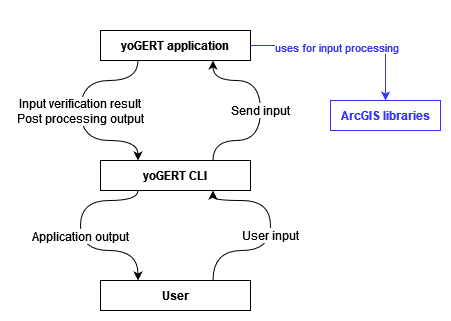
\includegraphics[width=0.6\linewidth]{REV0/SystDesign/sysdestcontextdiagram.png}
    \caption{System Context Diagram}
    \label{fig:System_Context_Diagram}
\end{figure}


\newpage
\section{Project Overview}

\subsection{Normal Behaviour}
Through the command line program of their choice (terminal, powershell, etc.), users will traverse to the yoGERT directory. From there, they will run the setup script within the home directory to update their environment and ensure correct version installation for all dependent libraries. Users may then use command line flags to upload their CSV GPS data for verification. after pre-processing and validating the data, the user can choose one of the following options:

\begin{itemize}
    \item[1.] Travel Episode Generation
    \item[2.] Identifying Activity Locations
    \item[3.] Generating Alternative Routes
\end{itemize}

After selection, users can choose the name, format, and directory of the file(s) outputted from the chosen operation. The user can then view the output in an external application, for example, Microsoft Excel for CSVs. 

\subsection{Undesired Event Handling}

%\wss{How you will approach undesired events}

\noindent A full analysis of the undesired event handling in the system can be found in the \href{../../HazardAnalysis/HazardAnalysis.pdf}{Hazard Analysis} document.\\

\noindent The main methods to handle undesired events are:
\begin{itemize}
    \item Robust documentation to help the user avoid any unauthorized or undefined actions
    \item A startup script to standardize the user's environment before running the toolbox
    \item Warnings provided to the user in the case of external environment factors (eg. too little memory for storage)
    \item Saving system state to avoid losing user data
\end{itemize}

\noindent If unexpected behaviour occurs, users will see error messages with recommended courses of action on their CLI. 

\subsection{Component Diagram}

\subsection{Connection Between Requirements and Design} \label{SecConnection}

\wss{The intention of this section is to document decisions that are made
  ``between'' the requirements and the design.  To satisfy some requirements,
  design decisions need to be made.  Rather than make these decisions implicit,
  they are explicitly recorded here.  For instance, if a program has security
  requirements, a specific design decision may be made to satisfy those
  requirements with a password.}

\section{System Variables}
\noindent N/A
%\wss{Include this section for Mechatronics projects}

\subsection{Monitored Variables}

\subsection{Controlled Variables}

\subsection{Constants Variables}

\section{User Interfaces}

\wss{The User Interface will consist of the command line interface along with HTML generated maps because the primary users of this tool are familiar with using the CLI and it'll be faster and more flexible for their needs than any GUI component that may constrict or narrow their usage scenarios. The HTML maps are highly interactive and responsive showing the output of the modules in detail. The stakeholder of this project also mentioned that the primary users would prefer CLI over GUIs}

\section{Design of Hardware}
\noindent N/A

\section{Design of Electrical Components}
\noindent N/A

\section{Design of Communication Protocols}
Communication protocols


\newpage
\section{Timeline}

\begin{table}[H] 
	\begin{tabularx}{\textwidth}{|X|X|X|}
		\hline
		\textbf{Module} & \textbf{Main Developer(s)} & \textbf{Due Date}\\
		\hline
		Input Pre-processing & Moksha Srinivasan & 
		January 24th, 2023  \\
		\hline
		Travel Episode Generation & Nicholas Lobo & 
		January 24th, 2023 \\
		\hline
		Mapping Module & Niyatha Rangarajan &
		January 28th, 2023 \\
		\hline
		Route Choice Generation & Abeer Al-Yasiri &
		January 29th, 2023 \\
		\hline
		Activity Location Detection & Smita Singh &
		January 30th, 2023 \\
		\hline 
		Travel Mode Detection & Nicholas Lobo & 
		January 30th, 2023 \\
		\hline 
		User Documentation & Longwei Ye &
		January 30th, 2023 \\
		\hline
		Setup Script & Moksha Srinivasan &
		January 31st, 2023 \\
		\hline 
	    Final Peer Code Reviews* & All &
		January 31st, 2023 \\
		\hline
		Integration Testing & Niyatha Rangarajan &
		February 1st, 2023 \\
		\hline
		Benchmark/Stress Testing & Longwei Ye & 
		February 2nd, 2023 \\
		\hline
	\end{tabularx}
	\caption{Module Timeline}
\end{table}

Before merging code, all team members will have written unit tests for their respective modules with mocked versions of the input ensuring correct module functionality. \\

\noindent *Note: Although code reviews have been taking place throughout the implementation process, the team plans to come together and review code once again before the final demonstration. This ensure that code and documentation is all up to date and in line with changing requirements. 



% \bibliographystyle {plainnat}
% \bibliography{../../../refs/References}

\newpage{}

\appendix

\section{Interface}

\wss{Include additional information related to the appearance of, and
interaction with, the user interface}

\section{Mechanical Hardware}
\noindent N/A
\section{Electrical Components}
\noindent N/A
\section{Communication Protocols}
communication
\section{Reflection}

\noindent One limitation of yoGERT is the use of the OSM database to retrieve data regarding transportation networks, activity locations, and general up-to-date GPS data. Since the dataset is crowd-sourced, it is not updated as often as say, Google Maps and the toolbox with subsequently have inaccuracies. With unlimited resources, the yoGERT team would aggregate data from alternative sources such as the most recently updated local transportation maps to increase accuracy. \\

\noindent Furthermore, another limitation of the solution provided is the CLI interface. With more time and resources the team would be keen to create a front-end interface that is accessible to a wide variety of users. This is because a CLI tool can have a very high barrier to entry for non-technically oriented stakeholders. Furthermore, a GUI tool could more easily help students and those keen to learn about geoprocessing visualize the output.\\

\noindent Finally, one big limitation in our design of yoGERT is the inability to append to existing inputs and outputs. Since the system is batch sequential, in the current implementation it is not able to quickly update inputs and add new episodes. This functionality is achievable and very useful, but would require an overhaul of the current design to succeed. \\

\noindent Another design that the team explored was embedding the application into a Jupyter notebook. This aided in the mission of yoGERT being a learning tool, with full code transparency and markdown comments throughout. This allowed the user to understand exactly what is occuring as they run the code and gain an intuitive understanding of how to process and manipulate GPS data. However, the main drawback of this approach is that Jupyter notebook can be slow to start up and take a long time to execute code. One of the main goals of the toolbox is the ability to quickly process large amounts of data which is difficult using Jupyter notebook. The developers chose to stick with a CLI interface as it is significantly faster and those who are interested can still look through the documentation and manipulate the code accordingly. \\

\noindent Lastly, the team also explored using R to implement the toolbox. This was an idea suggested by the team's supervisor due to the language being designed for large scale data manipulation. The benefits of R would have been the ability to complete deep statistical analysis which is very useful for route choice analysis and mode detection. The disadvantages are that R has significantly fewer libraries for our use case (geography) and visualizations tend to be more robust in python. On the contrary, python is less efficient for deep statistical analysis but has significantly more libraries for our use case, and it is easier to provide interactive data visualizations. \\

\end{document}